%        Fil: dokumentation.tex
%     Created: Mon Nov 13 22:45 PM 2011 C
% Last Change: Mon Nov 13 22:45 PM 2011 C
%
\documentclass[11pt,a4paper]{article}

% german dictionary
\usepackage[ngerman]{babel}

% enconding
\usepackage[utf8]{inputenc}

% graphics
\usepackage{graphicx}

% handle positions
\usepackage{float}

% additional math stuff
\usepackage{amsmath,amssymb,environ,esdiff,mathtools}

% set borders
\usepackage{a4wide}

% use URLs
\usepackage{url}

% expand table formatting
\usepackage{array}

% describe algorithms
\usepackage{algorithm}
\usepackage{algorithmic}

% header and footer
\usepackage{fancyhdr}
\pagestyle{fancy}
\fancyhf{}

\fancyhead[L]{Implementation einer Win/Win Strategie für das TSP}
\fancyhead[R]{Semesterarbeit}

\fancyfoot[L]{Andreas Brönnimann}
\fancyfoot[C]{\thepage}
\fancyfoot[R]{\today}
\renewcommand{\footrulewidth}{0.5pt}

% cover
\title {Semesterarbeit\\
Implementation einer Win/Win Strategie für das TSP\\}
\author {Andreas Brönnimann\\
Hochschule für Technik Zürich\\
Dozent: Dr. Hans-Joachim Böckenhauer}
\date {\today}

\begin{document}

% show all references, even the uncited ones
\nocite{*}

% show cover
\maketitle
\setcounter{page}{0}
\thispagestyle{empty}
\newpage

\tableofcontents
\newpage
\section{Einleitung}
\subsection{Ziel und Vorgehensweise}
Ziel dieser Arbeit ist es, die Win/Win Strategie des Papers "`Structural properties of hard metric TSP inputs"'\cite{moemke11} zu Implementieren. Anschliessend wird die Implementation zur Berechnung verschiedener Problemstellungen verwendet. Das Ergebnis wird mit den theoretisch erwarteten Resultaten verglichen und ausgewertet.

Um ein Verständnis für die Implementation zu entwickeln, werden das Traveling Salesman Problem (TSP oder übersetzt: das Problem des Handlungsreisenden), die Grundlagen von Win/Win Strategien und die verwendeten Algorithmen vorgestellt. 

Danach werden die wichtigsten Teile der Implementation erklärt, bevor dann die Ergebnisse ausgewertet werden. 

\subsection{Abgrenzung}
Diese Arbeit beschränkt sich auf die Implementation der Win/Win Strategie und die Auswertung der Ergebnisse. Neue Algorithmen zu finden ist nicht Teil dieser Arbeit.

\subsection{Motivation}
Mich fasziniert, dass die Problembeschreibung sehr einfach ist, die Lösung jedoch äusserst schwierig.
Ausserdem lassen sich viele Überlegungen mit Papier und Stift aufzeichnen, ohne das ein Computer benötigt wird. 
Abbildung \ref{img:simple_tsp} zeigt ein einfaches 6 Städte TSP, eine Mögliche Route ist dabei blau markiert. Offensichtlich ist es nicht die optimale Route. Das Bild zeigt jedoch, wie einfach man das Problem für kleine Instanzen analysieren kann, selbst ohne einen Rechner zu benutzen.

\begin{figure}[H]
        \centering
        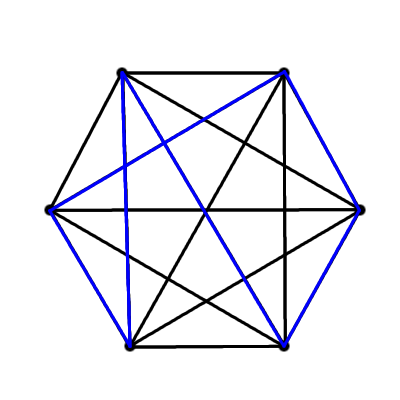
\includegraphics[width=8cm]{gfx/simple_tsp}
        \caption{einfaches 6 Städte TSP}
        \label{img:simple_tsp}
\end{figure}

\newpage
\section{Traveling Salesman Problem (TSP)}
\subsection{Problembeschreibung}
\subsection{Geschichte}
Der Urheber der Bezeichnung "`Traveling Salesman Problem"' ist nicht genau bekannt. Es ist jedoch klar, dass damit das Auffinden der kürzesten Rundreise eines Handelsreisenden gemeint ist.\footnote{vgl. \cite{applegate06} Seite 1-3} 1983 publizierte Heiner Müller-Merbach in seinem Paper\cite{mueller83} einen Ausschnitt aus dem Buch "`Der Handlungsreisende – wie er sein soll und was er zu thun hat, um Aufträge zu erhalten und eines glücklichen Erfolgs in seinen Geschäften gewiß zu sein – von einem alten Commis-Voyageur"' in dem die Wichtigkeit einer guten Route beschrieben:  
\begin{quotation}
Die Geschäfte führen Handlungsreisende bald hier, bald dort hin, und es lassen sich nicht füglich Reiserouten angeben, die für alle vorkommende Fälle passend sind: aber es kann durch eine zweckmäßige Wahl und Eintheilung der Tour, manchmal so viel Zeit gewonnen werden, dass wir es nicht glauben umgehen zu dürfen, auch hierüber einige Vorschriften zu geben. Ein Jeder möge so viel davon benutzen, als es seinem Zwecke für dienlich hält: so viel glauben wir aber davon versichern zu dürfen, daß es nicht wohl thunlich sein wird, die Touren durch Deutschland in Absicht der Entfernungen und, worauf der Reisende hauptsächlich zu sehen hat, des Hin- und Herreisens, mit mehr Oekonomie einzurichten. Die Hauptsache besteht immer darin: so viele Orte wie möglich mitzunehmen, ohne den nämlichen Ort zweimal berühren zu müssen.
\end{quotation}

Auch wenn das Problem in diesem Buch nicht mathematisch analysiert wird, beschreibt der Text das Traveling Salesman Problem. 

Eine der ersten mathematischen Analysen des Problem stammen aus dem Jahr 1757 vom berühmten Schweizer Mathematiker Leonard Euler. Er veröffentlichte ein Paper, in dem er eine Lösung zur "`Knights Tour"' vorstellte. Bei der "`Knights Tour"' soll auf einem Schachbrett mit dem Springer eine Folge von Sprüngen gefunden werden, so dass jedes Feld genau einmal besucht wird und der Springer am Ende wieder auf seinem Startfeld steht.

Dieses Problem kann als TSP formuliert werden. Die Wegkosten zu den mittels einem Springer erreichbaren Felder sind 0, die Kosten zu den nicht erreichbaren Felder sind 0.\footnote{vgl. \cite{applegate06} Seite 8-10}

\medskip

Einer der bedeutensten frühen Forscher auf dem Gebiet, Merril Flood, sagte in einem Interview, dass der Begriff "`Traveling Salesman Problem"' in den 1930er Jahren als Synonym für das "`48 States Problem"' von Hassler Whitney an der Princeton Universität verwendet wurde. Wer genau die Bezeichnung eingeführt habe, wisse er jedoch nicht.\cite{interview_merrill_flood84}

Abschliessend ist somit nicht auszumachen, wann genau die Forschung auf dem Gebiet des Traveling Salesman Problems begonnen hat.

%TODO: Beschreibung der Forschung 1960-heute

\newpage

\subsection{NP-Vollständigkeit}
Das Traveling Salesman Problem ist eines der bekanntesten NP\footnote{Nondeterministic Polynomial-Time}-Vollständigen Probleme. 

Es wird auch in der Liste von Karps 21 NP-Vollständigen Problemen aufgeführt. Die 1972 veröffentlichte List\cite{karp72} enthält sowohl das gerichtete, wie auch das ungerichtete Hamiltonkreisproblem (das TSP ist ein Spezialfall des Hamiltonkreisproblem). 

\medskip

In Hopcrofts "`Einführung in die Automatentheorie, formale Sprachen und Komplexitätstheorie"' findet sich folgende Definition:\footnote{\cite{hopcroft02} Seite 432}

Sei $L$ eine Sprache (eine Problem) in $\mathcal{NP}$. Wir sagen $L$ ist NP-vollständig, wenn folgende Aussagen über $L$ wahr sind:
\begin{itemize}
    \item L ist in $\mathcal{NP}$ enthalten.
    \item Für jede Sprache $L'$ in $\mathcal{NP}$ existiert eine polynomiale Reduktion von $L'$ auf $L$.
\end{itemize}

%TODO: Genauere Beschreibung, warum TSP NP-Vollständig
%Oder anders ausgedrückt: Wenn wir von einem Problem $L$ wissen, dass es in $\mathcal{NP}$ ist und wir unser Problem $P$ mit polynomialen Zeitaufwand auf das Problem $L$ abbilden können, dann ist $P$ NP-vollständig.

\subsection{Modellierung}
Das Problem des Handlungsreisenden wird für diese Arbeit (wie in vielen anderen Beispielen) als Graph modelliert. Dabei repräsentieren die Knoten die Städte und die Kanten die Kosten um von einer Stadt zur nächsten zu gelangen. Dabei sind die Kosten um von $A$ nach $B$ zu gelangen äquivalten zu den Kosten von $B$ nach $A$, es handelt sich also um einen ungerichteten Graphen.

Da alle Möglichen Routen berücksichtigt werden müssen, wird ein Vollständiger Graph verwendet, d.h. jeder Knoten ist mit jedem Knoten verbunden.

\subsection{Lösungsverfahren}
Neben dem hier vorgestellten Algorithmus existieren viele weitere Lösungsverfahren. Zum Vergleich sollen einige dieser Verfahren kurz vorgestellt werden.

\subsubsection{Exakte Lösungsverfahren}
\begin{flushleft}
\textbf{Brute Force}

Bei dieser Methode werden alle möglichen Kombinationen berechnet, bei jeder Berechnung wird verglichen, ob die Lösung besser ist, als die bisher berechneten Lösungen. Offensichtlich ist dieses Vorgehen äusserst ineffizient. Für 20 Städte müssen 2'432'902'008'176'640'000 (20!) Permutationen berechnete werden, dies entspricht $\approx$ $10^{18}$, also $\approx2.5$ Trillionen Möglichkeiten. Das Lösungsverfahren hat somit eine Laufzeit von $\mathcal O(n!)$.
%TODO: Genauere Ausführung: symmetrisch, asymmetrisch

\end{flushleft}

\medskip

\begin{flushleft}
\textbf{Branch-and-Cut}

\end{flushleft}

\medskip

\begin{flushleft}
\textbf{Held-Karp Algorithmus}
\end{flushleft}

\subsubsection{Heuristische Lösungsverfahren}
\begin{flushleft}
\textbf{Nearest-Neighbor-Heuristik}

\end{flushleft}

\medskip

\begin{flushleft}
\textbf{Ant Colony Optimization}

\end{flushleft}

\medskip

\begin{flushleft}
\textbf{MST-Heuristik}

\end{flushleft}
\newpage
\section{Win/Win Strategie}
\subsection{Grundidee}
\subsection{Anwendung für das Traveling Salesman Problem}
\newpage
\section{Algorithmen}
%TODO: Notation bei der beschreibung der Algorithmen vereinheitlichen
Der verwendete Algorithmus berechnet sowohl den Hamiltonpfad, wie auch den Hamiltonkreis für einen gegebenen Graphen $G$. 

Die Berechnung basiert auf dem Paper "`Structural Properties of Hard Metric TSP Inputs"'\cite{moemke11} (der Algorithmus wurde bereits im Paper "`Improved Approximations for TSP with Simple Precedence Constraints"'\cite{boeckenhauer10} vorgestellt):

\begin{algorithm}
    \caption{Hamiltonpfad und -kreis \cite{moemke11}}
    \label{alg:hp_hc}
\textbf{Eingabe:} Ein vollständiger Graph $G = (V,E)$, eine metrische Kostenfunktion $c: E \rightarrow \mathbb{Q}^+$ und zwei Knoten $s$ und $t$.
    \begin{enumerate}
        \item Minimalen Spannbaum $T$ von $G$ berechnen.
        \item Minimales Perfect Matching $M_C$ der ungeraden Knoten des minimalen Spannbaumes $T$ von $G$ berechnen.
        \item Minimales Perfect Matching $M_P$ der ungeraden Knoten des Multigraphen $T$ + \{$s$, $t$\} von $G$ berechnen.
        \item Die Eulertour Eul$_C$ des Multigraphen T $\cup$ $M_C$ und den Eulerpfad Eul$_P$ des Multigraphen T $\cup$ $M_P$ berechnen.
        \item Eul$_C$ zu einer Hamiltontour $H_C$ und Eul$_P$ zu einem Hamiltonpfad $H_P$ kürzen.
    \end{enumerate}
\textbf{Ausgabe:} $H_C$ and $H_P$.

\end{algorithm}

Nachfolgend werden die einzelnen Schritte des Algorithmus \ref{alg:hp_hc} genauer beschrieben. Dabei wird erläutert, welcher Algortihmus für den jeweiligen Schritt verwendet wird und wie dieser funktioniert.

\subsection{Eingabe}
Für die Berechnung wird ein vollständiger Graph erstellt, d.h. jeder Knoten des Graphen ist mit jedem anderen Knoten verbunden.

Damit der Hamiltonpfad berechnet werden kann, wird ein Startpunkt $s$ und ein Endpunkt $t$ benötigt.

\subsection{Minimaler Spannbaum - Algorithmus von Prim}
Auf dem als Eingabe erstellten vollständigen Graphen wird nun ein minimaler Spannbaum (MST) berechnet. Zur Berechnung des MST wird der Algorithmus von Prim genutzt.

Um den minimalen Spannbaum zu finden werden folgende Schritte abgearbeitet\footnote{vgl. \cite{cormen07} Seiten 574-577}:

%TODO: Wie soll der Algorithmus beschrieben werden?
\begin{algorithm}[H]
    \renewcommand{\algorithmicrequire}{\textbf{Eingabe:}}
    \renewcommand{\algorithmicensure}{\textbf{Ausgabe:}}
    \caption{minimaler Spannbaum}

    \begin{algorithmic}[1]
    \REQUIRE Ein vollständiger Graph $G$
        \STATE Wähle einen zufälligen Startknoten $v_0$ aus $G$
        \STATE Suche die Kante $e_0$ mit dem minimalen Gewicht, die mit $v_0$ verbunden ist (falls mehrere mit $v_0$ verbindene Kanten das minimale Gewicht aufweisen, wähle zufällig eine aus)
        \STATE Füge $e_0$ zum minimalen Spannbaum $M$ hinzu
        \STATE Entferne die Kante $e_0$ aus $G$

        \WHILE{$E(G) \ge 0$}
            \STATE Suche die Kante $e_n$ mit dem minimalen Gewicht, die mit $M$ verbunden ist (falls mehrere mit $M$ verbindene Kanten das minimale Gewicht aufweisen, wähle zufällig eine aus)
            \STATE Füge $e_n$ zum minimalen Spannbaum $M$ hinzu
            \STATE Entferne die Kante $e_n$ aus $G$
        \ENDWHILE
    \ENSURE minimaler Spannbaum $M$
    \end{algorithmic}
\end{algorithm}

%TODO: Bilder einfügen, um die Vorgehensweise aufzuzeigen?

\subsection{Minimales Perfektes Matching - Blossom V}
%TODO: Genauer beschreiben
Das minimale Perfekt Matching wird mittels Blossom V Algorithmus berechnet. Der Blossom V Algortihmus ist eine Weiterentwicklung des bekannten Blossom Algorithmus, der 1965 von Edmonds vorgestellt wurde.
Für diesen Algorithmus wird eine bestehende Implementation verwendet. 

\subsection{Eulerkreis - Hierholzer}
Die Berechnung des Eulerkreises wird mittels Algorithmus von Hierholzer zurück. Dieser wurde 1873 in der postum veröffentlichten Arbeit "`Über die Möglichkeit, einen Linienzug ohne Wiederholung und ohne Unterbrechung zu umfahren"'\cite{hierholzer73} beschrieben.

Der Algorithmus basiert auf der Idee, dass, wenn man in einem eulerschen Graphen einen beliebigen Kreis findet, die verbleibenden Kanten wiederum einen Kreis enthalten. Somit werden die gefundenen Kreise zusammengefügt, bis schlussendlich alle Kanten im Kreis enhalten ist und somit der Eulerkreis gefunden wurde.\footnote{vgl. \cite{krumke05} Seiten 46-48}

%TODO: Ist die beschreibung verständnlich?
\begin{algorithm}[H]
    \renewcommand{\algorithmicrequire}{\textbf{Eingabe:}}
    \renewcommand{\algorithmicensure}{\textbf{Ausgabe:}}
    \caption{Algorithmus von Hierholzer}

    \begin{algorithmic}[1]
    \REQUIRE Graph $G$, dessen Knoten alle einen geraden Grad aufweisen
        \STATE Wähle einen beliebigen Startknoten $v_0$
        \STATE Erstelle einen Kreis $K$ ausgehend von $v_0$
        \STATE Entferne alle Kanten von $K$ aus $G$
        \WHILE{$E(G) \ge 0$}
            \STATE Suche Knoten $v_n$ dessen Grad $\ge 0$
            \STATE Erstelle einen Kreis $K_n$ ausgehend von $v_n$
            \STATE Füge $K_n$ zu $K$ hinzu: Alle Knoten von $K_n$ an Stelle des Startknotens von $K_n$ in der korrekten Reihenfolge in $K$ einfügen
            \STATE Entferne alle Kanten von $K_n$ aus $G$
        \ENDWHILE
    \ENSURE Eulerkreis $K$
    \end{algorithmic}
\end{algorithm}

%TODO: Bilder einfügen, um die Vorgehensweise aufzuzeigen?


\subsection{Kürzung Eulerkreis/-pfad zu Hamiltonkreis/-pfad}
Die kürzung des Eulerkreises bzw. des Eulerpfades werden in der Liste der besuchten Knoten alle doppelten Einträge gelöscht.

\begin{algorithm}[H]
    \renewcommand{\algorithmicrequire}{\textbf{Eingabe:}}
    \renewcommand{\algorithmicensure}{\textbf{Ausgabe:}}
    \caption{Kürzung Eulerkreis/-pfad zu Hamiltonkreis/-pfad}

    \begin{algorithmic}[1]
    \REQUIRE Liste $L$ mit den Knoten des Eulerkreises/-pfades 
    \FOR{$i = 1 \to len(L)$}
        \IF{$L[i]$ not in $K$}
            \STATE Füge $L[i]$ zu $K$ hinzu
        \ENDIF
    \ENDFOR
    \ENSURE Hamiltonkreis/-pfad $H$
    \end{algorithmic}
\end{algorithm}

\newpage
\section{Implementation}
Der gesamte Algortihmus wurde in Python 3 implementiert. Lediglich der Blossom V Algorithmus, für welchen eine bestehende Implementation verwendet wurde ist in C++ implementiert.

Für die Knoten, Kanten und Graphen werden eigene Objekte erstellt, die nachfolgend genauer beschrieben werden. 

%TODO: Einleitung: Verwendete Programmiersprache, Unittesting, etc.
\subsection{Datenstrukturen}
\subsubsection{Knoten}
\subsubsection{Kante}
\subsubsection{Graph}
%TODO: Gewichte sind immer int Werte, verweis auf TSPLIB Doku
\subsubsection{Unittests}
\subsection{Minimaler Spannbaum}
\subsubsection{Eulerkreis}

\newpage

\section{Berechnungen}
\subsection{Vorgehen}

\subsection{Concorde}
Zur Berechnung der exakten Lösung wird die Software Concorde verwendet. Concorde wurde von David Applegate, Robert E. Bixby, Vašek Chvátal und William J. Cook, den Autoren des Buches "`Traveling Salesman Problem"'\cite{applegate06}, geschrieben.

Es ist sowohl möglich, die exakte Lösung zu berechnen, wie auch Heuristiken zu verwenden. Für diese Arbeit wurde lediglich die Berechnung der exakten Lösung verwendet.

Neben dem Kommandozeilen-Programm für Linux ist auch ein GUI für Windows verfügbar.\footnote{Download unter http://www.tsp.gatech.edu/concorde/downloads/downloads.htm}

\begin{figure}[H]
        \centering
        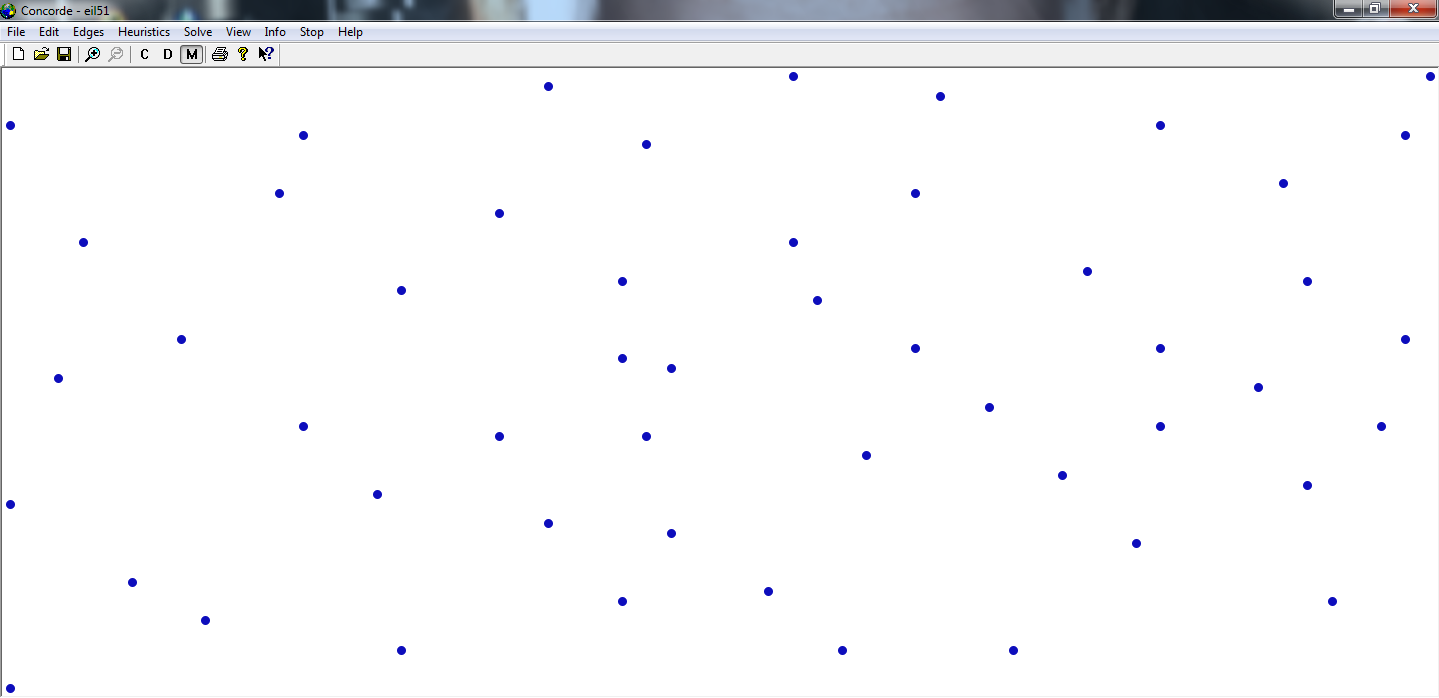
\includegraphics[width=11cm]{gfx/concorde_cities}
        \caption{Concorde stellt eil51 aus der TSPLIB garfisch dar}
        \label{img:concorde_cities}
\end{figure}

\begin{figure}[H]
        \centering
        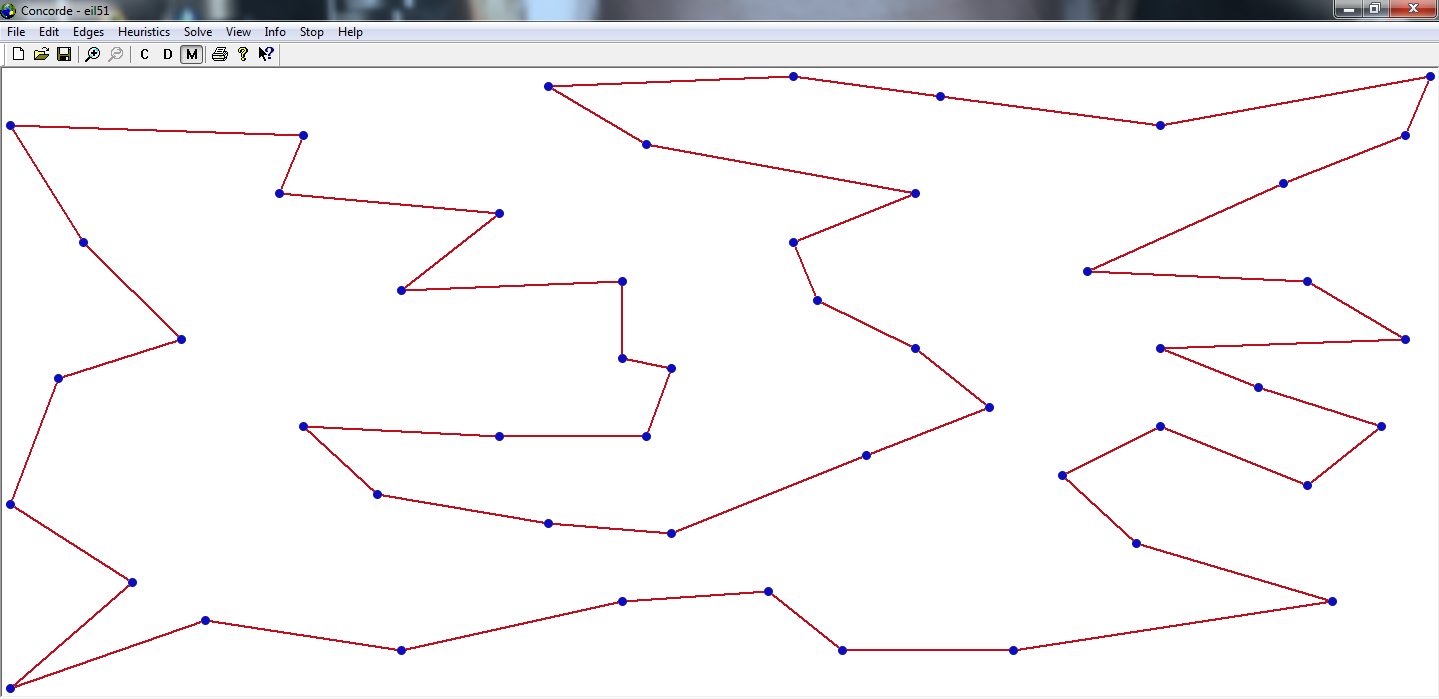
\includegraphics[width=11cm]{gfx/concorde_solution}
        \caption{Concorde hat die exakte Lösung zu eil51 berechnet}
        \label{img:concorde_solution}
\end{figure}

\subsection{TSPLIB}
\subsection{Zufällige Graphen}

\newpage

% bibliography
\bibliographystyle{plain}
\bibliography{bibliographie}
\end{document}
